\chapter{Estado del Arte}\label{chapter:state-of-the-art}

El proceso de construir modelos de \textit{machine learning} de gran calidad es complejo, iterativo y consume gran cantidad de tiempo, ya que este proceso está conformado por varios pasos. Los científicos de datos necesitan recolectar los datos y limpiarlos, seleccionar el algoritmo que mejor se ajuste a la tarea entre una cantidad enorme de algoritmos, ya sean técnicas de regresión, clasificación, de agrupamiento etc; además de afinar numerosos parámetros del algoritmo seleccionado y posteriormente aplicar numerosas métricas con el objetivo de juzgar el proceso de construcción del modelo. Por lo que la decisión del científico de dato en cada paso afecta directamente la construcción de un modelo de calidad, diferentes combinaciones de estos producen diferentes valores en las métricas que se evaluan. \\

Explorar todas las combinaciones posibles para resolver un problema muchas veces es no viable, ya que puede ser exponencial la cantidad de configuraciones en las cuales se puede evaluar nuestro problema, cada combinación conlleva al consumo de recursos computacionales y de tiempo. \\

La automatización de este proceso es llamado AutoML o Auto Machine Learning. Es importante saber que AutoML no es una tendencia nueva. En los años 1990s, soluciones comerciales ofrecían automatizar HPO para algoritmos de clasificación seleccionados vía \textit{grid search} \parencite{17}. Adaptaciones al \textit{grid search} para probar posibles configuraciones en un enfoque \textit{greedy} están disponibles desde 1995 \parencite{18}. Temprano en los 2000s las primeras estrategias eficientes para HPO fueron propuestas. Para configuraciones limitadas, por ejemplo afinar $C$ y $\gamma$ de un \textit{support vector machine} (SVM) \parencite{19} \parencite{20}, fue probado que las estrategias de búsqueda guiadas tienen mejor resultado que \textit {grid search} en menor tiempo. También en el 2004, el primer enfoque para automatizar la selección de características fue publicado \parencite{21}. Selección completa del modelo \parencite{22} fue el primer intento de construir automáticamente un pipeline de ML completo seleccionando un algoritmo de preprocesamiento, de selección de características y de clasificación simultáneamente, mientras se afinaban los hiperparámetros de cada uno de estos algoritmos. Evaluando este enfoque en varios conjuntos de datos se demostró el potencial de este método \parencite{23}. Iniciando el 2011 muchos métodos diferentes aplicando optimización Bayesiana para la afinación de hiperparámetros \parencite{24} \parencite{25} y selección de modelos fueron propuestos \parencite{13}. En el 2015, el primer método de ingeniería de características automático sin conocimiento del dominio fue propuesto \parencite{26}. Es posible construir pipelines de forma variable desde el 2016 \parencite{27}. En el 2017 y 2018 el tema de AutoML recibió mucha atención en los medios con la realización de soluciones comerciales de AutoML \parencite{28} \parencite{29} \parencite{30} \parencite{31}. Simultáneamente las investigaciones en el área de AutoML ganaron mucha atracción conllevando a mejoras de rendimiento significativas. Métodos recientes son capaces de reducir el tiempo de corrida de procedimientos AutoML desde varias horas a algunos minutos \parencite{32}.

\section{AutoML como problema CASH}

El AutoML como problema CASH o \textit{Combined Algorithm Selection and Hyperparameter Optimization} fue introducido por Auto-Weka el cual define dos procesos importantes en la etapa de AutoML, la selección del modelo(\textit{Model Selection}, ML) y la optimización de hiperparámetros (\textit{Hyperparameter Optimization}, HPO).

\subsection{Model Selection:}
Dado un conjunto de algoritmos de \textit{machine learning} $\mathcal{A}$ y una limitada cantidad de datos de entrenamiento $\mathcal{D} = \{(x_1, y_1), ..., (x_n, y_n)\}$ el objetivo de la selección del modelo es determinar el algoritmo $A^* \in \mathcal{A}$ con un desempeño general óptimo. El desempeño general es estimado dividiendo $\mathcal{D}$ en conjuntos disjuntos de entrenamiento y validación $\mathcal{D}^{i}_{train}$ y $\mathcal{D}^{i}_{valid}$, funciones $f_i$ que aprenden al aplicar $A^*$ a $\mathcal{D}^{i}_{train}$ y evaluar el desempeño predictivo de estas funciones en $\mathcal{D}^{i}_{valid}$. Esto permite escribir el problema de selección del modelo de la siguiente forma:

$$A^* \in \argmin_{A \in \mathcal{A}} \frac{1}{k} \sum^{k}_{i = 1} \mathcal{L}(A, \mathcal{D}^{i}_{train}, \mathcal{D}^{i}_{valid}) $$
Donde $\mathcal{L}(A, \mathcal{D}^{i}_{train}, \mathcal{D}^{i}_{valid})$ es la pérdida obtenida por $A$ cuando fue entrenada con $\mathcal{D}^{i}_{train}$ y evaluada en $\mathcal{D}^{i}_{valid}$.

\subsection{Hyperparameter Optimization:}
El problema de optimización de hiperparámetros $\lambda \in \Lambda$ de un algoritmo de \textit{machine learning} $A$ es conceptualmente similar al problema de selección del modelo. Algunas diferencias claves son que los hiperparámetros a menudo son valores contínuos, que el espacio de hiperparámetros es de grandes dimensiones y que se puede explotar la correlación entre distintas configuraciones de parámetros. Dados $n$ hiperparámetros $\lambda_1, ..., \lambda_{n}$ con dominios $\Lambda_1, ..., \Lambda_n$ el espacio de hiperparámetros $\lambda$ es un subconjunto del producto cruzado de estos dominios $\Lambda \subset \Lambda_1 \times ... \times \Lambda_n$. Este subconjunto es a menudo estricto, tal que algunas configuraciones de hiperparámetros hacen inactivos a otros hiperparámetros. Más formalmente, se dice que un hiperparámetro $\lambda_i$ es condicional en otro hiperparámetro $\lambda_j$ si $\lambda_i$ está activo si el hiperparámetro $\lambda_j$ toma valores en un conjunto dado $V_i(j) \subset \Lambda_j$. Dando lugar a un espacio en forma de árbol o algunas veces en forma de grafo dirigido acíclico(DAG). Dado un espacio $\Lambda_{A}$ el problema de optimización de hiperparámetros puede ser escrito como:
$$\lambda^* \in \argmin_{\lambda \in \Lambda} \frac{1}{k} \sum^{k}_{i = 1} \mathcal{L}(A_{\lambda}, \mathcal{D}^{i}_{train}, \mathcal{D}^{i}_{valid}) $$.

\section{Componentes del proceso de AutoML}
En el proceso de AutoML destacan tres tareas importantes, la primera es el espacio de búsqueda el cual representa el conjunto de todas las posibles combinaciones que pueden resolver nuestro problema, la segunda es la estrategia de búsqueda que tiene como objetivo encontrar soluciones en el espacio de búsqueda de forma óptima y la tercera es la métrica de rendimiento que se utiliza para comparar que tan buena puede ser una solución con respecto a otra.

\subsection{Espacio de búsqueda}
La búsqueda de espacio define un paradigma estructural que los métodos de optimización de arquitecturas pueden explorar, por lo que diseñar un buen espacio de búsqueda es un problema retador de vital importancia. En general de un buen espacio de búsqueda se espera que excluya el sesgo humano y que sea lo suficientemente flexible para cubrir una gran variedad de arquitecturas de modelos.

Un espacio de búsqueda relativamente sencillo es el espacio de redes neuronales con estrucutra de cadenas(\textit{chain-structured neural network}). Una arquitectura de red neuronal con estructura de cadena puede ser escrita como una secuencia de capas, donde la $i$-th capa $L_i$ recibe en su entrada la salida de la capa $L_{i-1}$, y su salida sirve como entrada de la capa $L_{i + 1}$. Entonces el espacio de búsqueda está parametrizado por:

\begin{itemize}
\item El máximo número de capas.
\item El tipo de operación que cada capa ejecuta.
\item Los hiperparámetros asociados con la operación (p.e. número de filtros, tamaño del kernel). Los parámetros son condicionados por lo que el espacio de búsqueda es condicional.
\end{itemize}

Trabajos recientes en NAS (\parencite{56} \parencite{65} \parencite{66} \parencite{67} \parencite{68}) incorporan elementos de diseño moderno conocidos como arquitecturas \textit{hand-crafted}, como conexiones de satlo que permiten construir redes de múltiples ramas. En este caso la entrada de la capa $i$ puede ser descrita como una función que combina la salida de capas anteriores. El empleo de tal función da como resultado más grados de libertad.\\

Consecuentemente, este espacio de búsqueda basado en celdas es también empleado exitosamente por muchos trabajos recientes \parencite{68} \parencite{37} \parencite{62} \parencite{67} \parencite{69}. Sin embargo, surge una nueva elección de diseño cuando se utiliza un espacio de búsqueda basado en celdas, cómo elegir la macroarquitectura: ¿cuántas celdas se utilizarán y cómo se conectarán para construir el modelo real. Por ejemplo, \parencite{56} construyen un modelo secuencial a partir de celdas, en el que cada celda recibe como entrada las salidas de las dos celdas anteriores, mientras que \parencite{69} emplean la estructura de alto nivel de arquitecturas conocidas manualmente diseñadas, como DenseNet \parencite{70}, y usan sus celdas dentro de estos modelos. Un paso en la dirección de optimizar las macroarquitecturas es el espacio de búsqueda jerárquico introducido por \parencite{38}, que consta de varios niveles de motivos. El primer nivel consta del conjunto de operaciones primitivas, el segundo nivel de diferentes motivos que conectan operaciones primitivas a través de un DAG, el tercer nivel de motivos que codifican cómo conectar motivos de segundo nivel, y así sucesivamente. El espacio de búsqueda basado en celdas puede verse como un caso especial de este espacio de búsqueda jerárquico donde el número de niveles es tres, los motivos del segundo nivel corresponden a las celdas y el tercer nivel es la macroarquitectura codificada. \\
La elección del espacio de búsqueda determina en gran medida la dificultad del problema de optimización: incluso para el caso del espacio de búsqueda basado en una sola celda con macroarquitectura fija, el problema de optimización sigue siendo discontinuo y con dimensiones relativamente altas.


\subsection{Estrategia de búsqueda}

Las técnicas de aprendizaje profundo constituyen un subconjunto de metodologías de \textit{machine learning} que son basadas en redes neuronales artificiales (ANN) las cuales principalmente fueron inspiradas en la arquitectura del cerebro humano \parencite{34}. Se describe como profundo porque tiene más de una capa de transformaciones de características no lineales. Búsqueda de arquitecturas neuronales (NAS) es un paso fundamental en la automatización de los procesos de \textit{machine learning} y ha sido exitosamente usado para el diseño de arquitecturas de modelos para imágenes y tareas del lenguaje \parencite{35} \parencite{36} \parencite{37} \parencite{38} \parencite{39}. Las técnicas NAS recaen en 5 principales categorías que incluyen, \textit{random search}, aprendizaje por reforzamiento, métodos basados en gradiente, métodos evolutivos y métodos de optimización Bayesiana.

\begin{figure}[H]
    \center 
    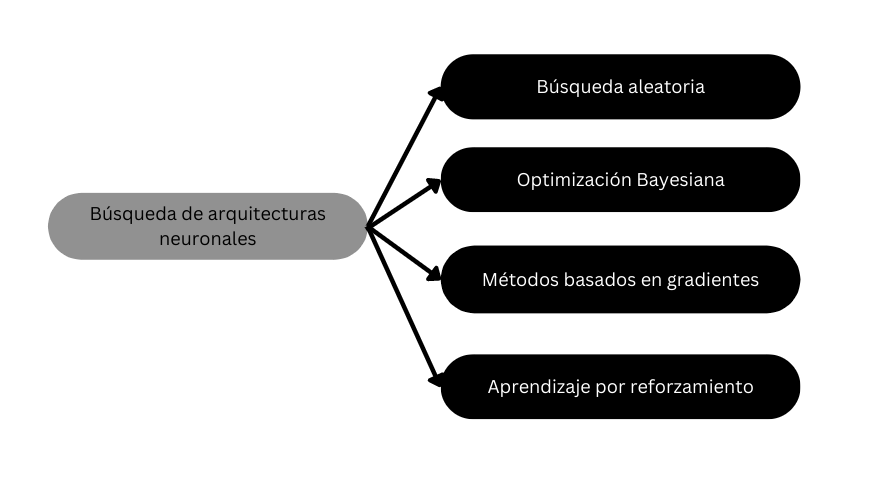
\includegraphics[scale=0.4]{images/NAS.png}
    \caption{Técnicas de arquitecturas de redes neuronales}
\end{figure}

\textit{Random search} es uno de los enfoques más ingenuos y simples para la búsqueda de arquitectura de red. Por ejemplo, \parencite{40} han presentado un enfoque para encontrar una buena arquitectura de red mediante la búsqueda aleatoria combinada con un conjunto bien entrenado de pesos compartidos. \parencite{41} propusieron nuevas líneas de base de búsqueda de arquitectura de red que se basan en la búsqueda aleatoria con parada anticipada para la optimización de hiperparámetros. Los resultados muestran que la búsqueda aleatoria junto con la parada anticipada logra resultados de búsqueda de arquitectura de red en el estado del arte en dos marcadores NAS estándar..

\textit{Reinforcement Learning} \parencite{42} es otro enfoque que se ha utilizado para encontrar la mejor arquitectura de red. \parencite{43} utilizaron una red neuronal recurrente (LSTM) con refuerzo para componer la arquitectura de la red neuronal. Más específicamente, la red neuronal recurrente se entrena a través de un algoritmo de búsqueda basado en gradiente llamado REINFORCE \parencite{44} para maximizar la precisión esperada de la arquitectura de la red neuronal generada. \parencite{45} introdujo un algoritmo de \textit{meta-modeling} llamado MetaQNN basado en el aprendizaje por refuerzo para generar automáticamente la arquitectura de la red neuronal convolucional para una nueva tarea. Las capas de la red neuronal convolucional son elegidas secuencialmente por un agente de aprendizaje que está entrenado usando \textit{Q-learning} con una técnica de exploración $\mathcal{E}$-\textit{greedy}. Simplemente, el agente explora un espacio de búsqueda finito de un conjunto de arquitecturas e iterativamente descubre diseños de arquitectura con un rendimiento mejorado en la nueva tarea a aprender.

\textit{Gradient-based optimization} es otra forma común para búsquedas de arquitecturas de redes neuronales. \parencite{46} propuso un enfoque basado en la relajación contínua de la arquitectura neuronal permitiendo usar descenso del gradiente para la búsqueda de la arquitectura. Los experimentos mostraron que este enfoque sobresale en encontrar arquitecturas convolucionales de alto rendimiento para la clasificación de imágenes en CIFAR-10, y en los conjuntos de datos de \textit{ImageNet}. \parencite{47} propuso un enfoque de optimización del descenso del gradiente para aprender la arquitectura de la red y parámetros simultáneamente. \parencite{48} usaron un enfoque basado en el gradiente para aprender arquitectura de redes. Los resultados experimentales en dos arquitecturas de redes diferentes: \textit{ResNet} y \textit{ResNeXt} mostraron que este enfoque recae en mejor precisión una reducción significativa en el número de parámetros. 

\textit{Bayesian optimization} basado en procesos \textit{Gaussian} ha sido usado por \parencite{49} y \parencite{50} para abordar el problema de búsqueda de arquitectura de redes neuronales. En adición, muchos trabajos se enfocaron en usar modelos basados en árboles como \textit{random forests} y \textit{tree Parzen estimators} \parencite{51} para efectivamente optimizar la arquitectura de red al igual que sus hiperparámetros \parencite{52} \parencite{53} \parencite{54}. La optimización Bayesiana  puede superar a algoritmos evolutivos en algunos problemas \parencite{55}

\subsection{Estrategia de rendimiento}
El objetivo de NAS es típicamente encontrar arquitecturas que puedan obtener alto rendimiento en la predicción de datos no vistos. La opción simple es ejecutar un entrenamiento estándar y la validación de la arquitectura en los datos, pero esto desafortunadamente es costoso computacionalmente y limita el número de arquitecturas que pueden ser exploradas. Investigaciones más recientes se enfocan en el desarrollo de métodos que reducen el costo de estas estimaciones de rendimiento. \\

El rendimiento puede ser estimado basado en \textit{lower fidelities} del actual rendimiento luego de un entrenamiento completo(también llamado \textit{proxy metrics}). Estas \textit{lower fidelities} incluyen menor tiempo de entrenamiento (\parencite{56} \parencite{57}), entrenar un subconjunto de los datos \parencite{58}, en imágenes de baja resolución \parencite{59}, o con menos filtros por capa y menos celdas. Mientras estas aproximaciones \textit{low-fidelity} reducen el costo computacional, también introducen un sesgo en la estimación, ya que normalmente se subestima el rendimiento. Esto puede que no sea problemático siempre que la estrategia de búsqueda solo se base en clasificar diferentes arquitecturas y la clasificación relativa permanezca estable. Sin embargo, resultados recientes indican que esta clasificación relativa puede cambiar drásticamente cuando la diferencia entre las aproximaciones baratas y la evaluación “completa” es demasiado grande \parencite{57}, lo que aboga por un aumento gradual de las fidelidades \parencite{60} \parencite{61}.\\

Otra estrategia aplicada con éxito a las redes neuronales convolucionales (Convolutional Neural Networks, CNN) es compartir pesos entre diferentes modelos, lo que se conoce como compartición de parámetros o compartición de pesos \parencite{62}. Para NAS diferenciables con un gran modelo one-shot, la compartición de parámetros se logra naturalmente ya que las arquitecturas y los pesos se entrenan conjuntamente. Sin embargo, entrenar el modelo one-shot puede ser difícil ya que contiene todas las operaciones posibles. Para acelerar aún más el proceso de entrenamiento, \textit{single-path one-shot} fue propuesto \parencite{63} en el que solo se activa una operación entre un par de entrada y salida durante cada paso. Para NAS sin un modelo \textit{one-shot}, compartir pesos entre diferentes arquitecturas es más difícil pero no del todo imposible. Por ejemplo, dado que se sabe que algunos filtros convolucionales son extractores de características comunes, heredar pesos de arquitecturas anteriores es factible y razonable en las CNN \parencite{64}. 



